\begin{titlepage}

\centering

\begin{tikzpicture}

\node[inner sep=0pt] (logo) at (0,0.65)
    {
\includegraphics[scale=0.05]{Figures/0. General/linux_penguin.png}};
{\setstretch{2.0}
\node[text width = 0.58\textwidth, yshift = 0.35cm, right = 1.25cm of logo](title){\sffamily\huge\reporttitle};
}   


\node[text width = 0.6\textwidth, xshift = 0.1cm, yshift = 0.5cm, below = 0.5cm of title](subtitle){\sffamily\Large \reportsubtitle};

\gettikzxy{(subtitle.south)}{\sffamily\subtitlex}{\subtitley}
\gettikzxy{(title.north)}{\titlex}{\titley}
\draw[line width=1mm, color_scheme]($(logo.east)!0.5!(title.west)$) +(0,\subtitley - 1cm) -- +(0,\titley - 0.55cm);

\end{tikzpicture}
\vspace{3.5cm}
% \sffamily\groupnumber

\begin{table}[H]
\centering
\sffamily
\large
\begin{tabu} to 2.8\linewidth{cc}
\textbf{Autores:}\\
\sffamily
\reportauthors
\end{tabu}

\end{table}

\sffamily \large \grouptutor

\tikz[remember picture,overlay]\node[anchor=south,inner sep=0pt] at (current page.south) {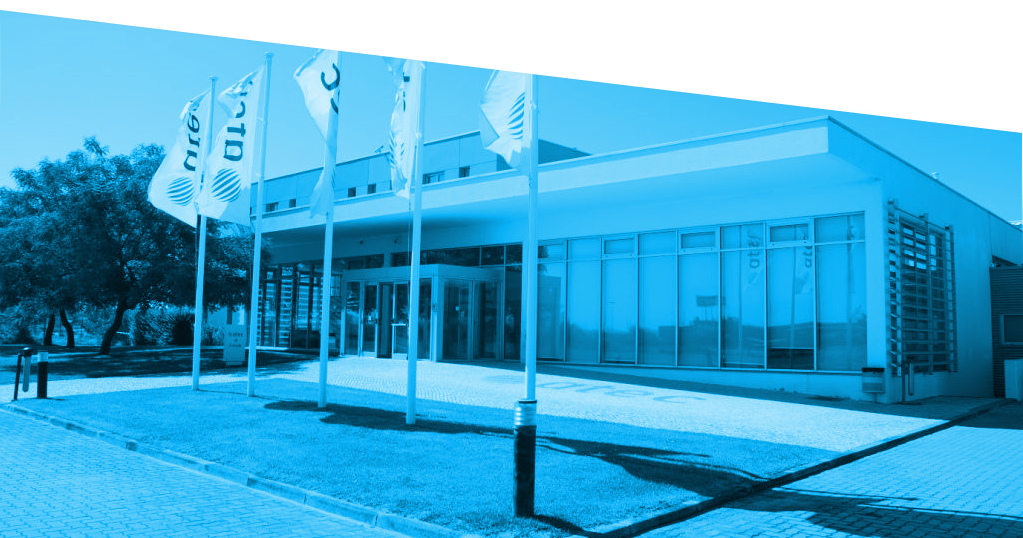
\includegraphics[width=\paperwidth]{Figures/0. General/atec.png}};

\mbox{}
\vfill
\begin{figure}[H]
    \centering
    \hspace{-0.5cm}
    \vspace{-0.5cm}
    % width=\textwidth para imagem da largura do texto
    
\includegraphics[scale=0.5]{Figures/0. General/atec_logo_white.png}
\end{figure}
\sffamily \LARGE \textcolor{white}{\placeanddate} \\



\end{titlepage}








